\documentclass{article}
\usepackage{amsmath,amssymb}
\usepackage[numbers]{natbib}
\usepackage{geometry}
 \geometry{
 a4paper,
 total={170mm,257mm},
 left=30mm,
 top=30mm,
 right=30mm,
 bottom=30mm
 }
 
\usepackage{graphicx}
\usepackage{caption}
\usepackage{subcaption}
\usepackage{float}

\usepackage{hyperref}
\hypersetup{%
  colorlinks=true,% hyperlinks will be coloured
}

\setlength{\parskip}{1em}

\title{Reinforcement Learning Assignment-5 \\
	\Large Function Approximation, Policy Gradients and Actor-Critic Methods \\}
\begin{document}
\author{Utkarsh Prakash \\ \normalsize 180030042}
\maketitle
\section{OpenAI Gym Environments Considered}
    \subsection{Mountain Car}
    A car is on a one-dimensional track, positioned between two "mountains". The goal is to drive up the mountain on the right; 
    however, the car's engine is not strong enough to scale the mountain in a single pass. Therefore, the only way to succeed is to 
    drive back and forth to build up momentum. \par

    \noindent %The next paragraph is not indented
    The state of the car is decided by the position of the car along the horizontal axis and the velocity. At the beginning of the
    episode, the car starts from the bottom of the hills (valley). The episode ends when the car reaches the goal or after
    200 steps (which ever is earlier). The action space consists of 3 actions: \{push left, push right, do nothing\}. A negative reward
    of $-1$ is applied at each timestep. The objective of the car is to reach the top of the hill on the right as early as possible, 
    because at each timestep it will be rewarded negatively. \par

    \begin{figure}[H]
        \graphicspath{ {../tmp/} }
        \begin{center}
        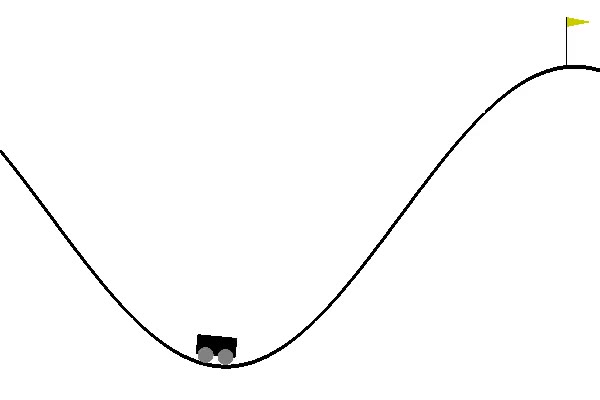
\includegraphics[width=8cm]{mountain_car.jpg}
        \end{center}
        \caption{MountainCar. For more details click \href{https://gym.openai.com/envs/MountainCar-v0/}{here} }
        \label{mountain_car}
    \end{figure}

    \subsection{CartPole}
    A pole is attached by an un-actuated joint to a cart, which moves along a frictionless track. The system is controlled by applying a 
    force of +1 or -1 to the cart. The pendulum starts upright, and the goal is to prevent it from falling over. A reward of +1 is provided for
    every timestep that the pole remains upright. The episode ends when the pole is more than 15 degrees from vertical, or the cart moves more 
    than 2.4 units from the center or the length of the episode is atleast 200.\par
    
    \begin{figure}[H]
        \graphicspath{ {../tmp/} }
        \begin{center}
        
\includegraphics[width=8cm]{cartpole.png}
        \end{center}
        \caption{CartPole. For more details click \href{https://gym.openai.com/envs/CartPole-v1/}{here} }
        \label{policy_iter_jack_problem}
    \end{figure}
    
    \noindent %The next paragraph is not indented
    The state of the cart is decided by it's position (x), velocity (x\_dot), pole angle (theta) and pole angular velocity (theta\_dot). The action space
    consists of 2 actions: \{push left, push right\}.

\section{Linear Function Approximation}
    \subsection{Mountain Car}
        \subsubsection{Tile Coding}
        We consider a grid of 14 x 14 tiling i.e. each tiling consists of 196 tiles and we have $n=7$ such tilings. The offsets for these tilings were:
        [(0, 0), (0.018, 0.004), (0.036, 0.008), (0.055, 0.013), (0.073, 0.017), (0.092, 0.021), (0.110, 0.025)], where the first and second dimension represents 
        the position and velocity of the car respectively. We run each of the algorithm for $5,000$ episodes and 
        average the results over $10$ runs. The $\epsilon$ or the exploration factor in the $\epsilon$-greedy policy is chosen to be $0.8$ initially and is 
        decreased by a factor of $0.99$ after every epsiode. This ensures that each of the state is explored infinitely often. The learning rate or the step-size 
        $(\alpha)$ and discount factor $(\gamma)$ are chosen to $0.3/n$, where $n$ is the number of tiling and $0.99$ respectively. We use a constant step-size.

        \subsubsection{Radial Basis Function Coding}

    \subsection{CartPole}
        \subsubsection{Tile Coding}
        We consider a hyper-grid of 22 x 22 x 22 x 22 tiling i.e. each tiling consists of $22^{4}$ tiles and we have $n=4$ such tilings. The offsets for these 
        tilings were: [(0, 0, 0, 0), (0.07, 0.23, 0.03, 0.55), (0.14, 0.48, 0.06, 1.11), (0.20, 0.71, 0.08, 1.67)], where the dimensions represent position (x), 
        velocity (x\_dot), pole angle (theta) and pole angular velocity (theta\_dot) of the cart respectively. We run each of the algorithm for $5,000$ episodes and 
        average the results over $10$ runs. The $\epsilon$ or the exploration factor in the $\epsilon$-greedy policy is chosen to be $0.8$ initially and is 
        decreased by a factor of $0.99$ after every epsiode. This ensures that each of the state is explored infinitely often. The learning rate or the step-size 
        $(\alpha)$ and discount factor $(\gamma)$ are chosen to $0.1/n$, where $n$ is the number of tiling and $0.99$ respectively. We use a constant step-size.

        \subsubsection{Radial Basis Function Coding}

\section{REINFORCE Algorithm}
    \subsection{Mountain Car}

    \subsection{CartPole}
    We parameterize the policy using a neural network consisting of 4, 16 and 2 units in the input, hidden and output layer. We use ReLU and softmax activation for
    the first and second layer respectively. We run each of the algorithm for $5,000$ episodes and average the results over $2$ runs. 
    The learning rate or the step-size $(\alpha)$ used is fixed and equals $0.01$. The discount factor $(\gamma)$ is chosen to be $0.99$. We compare the performance
    of versions of the REINFORCE algorithms which differ in their policy gradient calculation, as described below:
    \begin{equation}
        \nabla \rho(\theta) = \mathbb{E}_{\tau} \left [\left ( \sum_{t=0}^{T} \nabla_{\theta} log \pi (a_{t} | s_{t}) \right) \left ( \sum_{t=0}^{T} \gamma^{t} R_{t} \right) \right ]
    \label{reinforce}
    \end{equation}

    \begin{equation}
        \nabla \rho(\theta) = \mathbb{E}_{\tau} \left [\left ( \sum_{t=0}^{T} \nabla_{\theta} log \pi (a_{t} | s_{t}) \left ( \sum_{k=t+1}^{T} \gamma^{k-t-1} R_{k} \right) \right) \right ]
    \label{reinforce_variance}
    \end{equation}
    Let's call the version of the algorithm described by \ref{reinforce} and \ref{reinforce_variance} as \textbf{REINFORCE} and \textbf{REINFORCE\_var} respectively. 



\end{document}